\documentclass[10pt,letterpaper]{article}
\usepackage{tools}
\usepackage{enumitem}
%\settextfont{B Nazanin}
\usepackage{lipsum}
\setlength{\parskip}{3mm}
\setlength{\parindent}{0mm}
\begin{document}
\Large
\begin{center}
In the name of beauty

2nd problem set solution of ComNet course
\hl
\end{center}
Q1)

\begin{enumerate}[label=\alph*-]
\item
False. The UDP's freedom on imposing no congestion control can lead to packet loss in contrast to TCP, thereby reducing the effective throughput.
\item
True. Indeed a single file to share between users must be distributed between multiple devices according to the philosophy of Peer-to peer connection. The more users to share resourses, the better the application works.
\item
False. Yet the connection initiater and connection acceptor can be regarded as client and server, respectively.
\item
False. One IP addresses are referenced correctly, the Transport layer must address within which socket should it deliver the message to the Application layer. All in all, the socket number must be included.
\item
True. To that reason, cookies are a key solution to stateless HTTP servers.
%\item
%Link-layer switches are typically capable of processing the packets up to the layer 3.
%\item
%SMTP and FTP are examples of layer 1 protocols while TCP is a transport layer protocol.
%\item
%API is a set of rules 
%\item
%For economical reasons, exploiting optical fibers is not recommended in long-haul network
\end{enumerate}

Q2)

When clients make a DNS query for a name
mapped to a set of addresses, the server responds with the entire set of IP
addresses, but rotates the ordering of the addresses within each reply. Because a
client typically sends its HTTP request message to the IP address that is listed
first in the set, DNS rotation distributes the traffic among the replicated servers. The motivation is lowering the burden on the web server.

Q3)

Each image takes 80msec to be downloaded through the connection. In a non-persistent connection, the user client has to send two requests for each of the 5 images, yielding a total amount of $12\text{RTT}+5\times 80msec=412msec$ elapsed time. In a persistent connection however, the connection is established once at the first user request on retrieving the web page. The connection is torn down if the user client does not send any request during an interval. The total time would be $7\text{RTT}+5\times 80msec=407msec$.

Q4)

\textbf{\color{red}(There was an unintentional typo in the question. The ${\text{requests}\over \text{sec}}$ unit must have been replaced by ${\text{requests}}$ !)}

(Extra info: the intervening red square in the topology, is typically a layer-3 switch which processes the host demands)

a- The average request of the user 2 is
$$
{8+12\over 2}=10 {\text{requests}}
$$
hence, the upstream link would have to bear with a total of $
10+15=25 {\text{requests}}
$ or equivalently $200\text{Mbits}$ on average. The total Internet delay time would then be $$
{200\text{Mbits}\over 1\text{Mbps}}=200\text{sec}
$$
from which, the share of the users 1 and 2 is 120msec and 80msec, respectively.

b- By using the results of the previous parts, the total amount of $200\text{Mbits}$ would be satisfied by 40\% from the web cache (which would impose a delay of 8 sec) and by 60\% through the Internet with the corresponding delay of 120sec. The total delay is reduced from 200sec to 128sec which is divided into 76.8sec and 51.2sec for the users 1 and 2, respectively.

Q5)

By using the following formula:
$$
D_\text{p2p}\ge \max\left\{{F\over u_s},{F\over d_\text{min}},{NF\over u_s+\sum_{i=1}^nu_i}\right\}
$$
we would obtain
$$
D_\text{p2p}\ge\max\left\{{15\times 1000\over 30},{15\times 1000\over 2},{N\times 15\times 1000\over 30+Nu}\right\}=7500\cdot\max\left\{1,{2N\over 30+Nu}\right\}
$$
The following chart would conclude all the previous calculations:
\begin{figure}[h!]
\centering
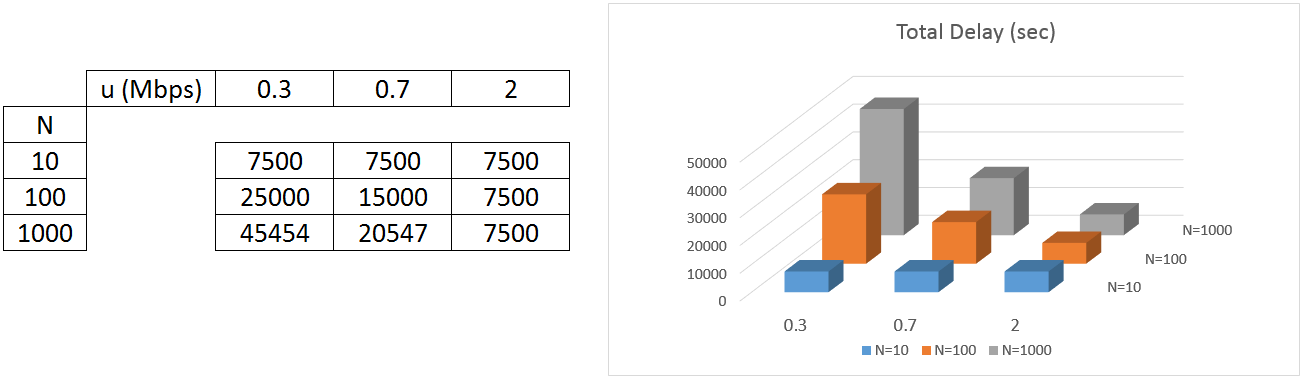
\includegraphics[width=170mm]{charthw2}
\end{figure}
%Consider distributing a file of $F$ = 15 Gbits to $N$ peers. The server has an upload
%rate of $u_s$ = 30 Mbps, and each peer has a download rate of $d_i$ = 2 Mbps and an
%upload rate of $u$. For $N$ = 10, 100, and 1,000 and $u$ = 300 Kbps, 700 Kbps, and
%2 Mbps, prepare a chart giving the minimum distribution time for each of
%the combinations of $N$ and $u$ for both client-server distribution and P2P
%distribution.
%
%(Hint: The distribution time is the time it takes to get a copy of the file to all $N$ peers. At the beginning of the distribution in P2P file sharing, only the server has the file. To get this file
%into the community of peers, the server must send each bit of the file at least once
%into its access link.)

%Consider the following network in which node A wants to send packets to node B through a router and two links:
%\begin{figure}[ht]
%\centering
%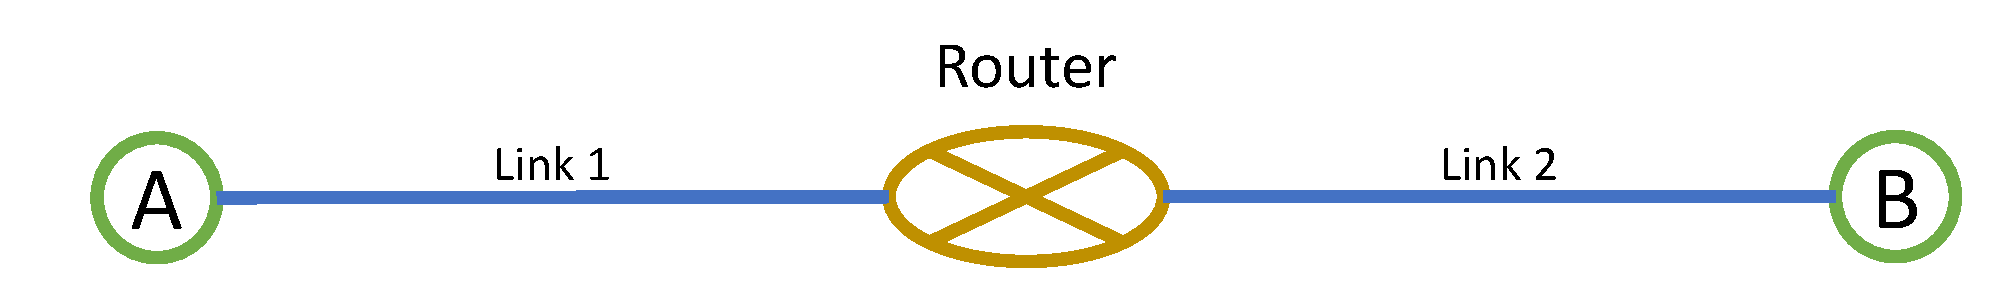
\includegraphics[width=140mm]{p2p}
%\end{figure}
%Assume the transmission rate of the links 1 and 2 to be 100Mbits/sec and 50Mbits/sec, respectively and both of the links be 10km long. The speed of light is $2\times 10^8$m/s in the links.
%\begin{enumerate}[label=\alph*-]
%\item
%What is the end-to-end propagation delay?
%\item
%Assume node A wishes to transmit 4 consecutive, 12.5Kbytes packets, each of which being sent at a single 1ms time slot, that is, packet 1 is sent in the first time slot, packet 2 is sent in the second time slot and so on. If the router does not impose processing delay on packets, how much buffer capacity would it need for storing incoming packets in the 4th time slot due to the queuing delay of the previously received packets?
%\item
%Is there any bottleneck link and if so, which one and why?
%\end{enumerate}
%
%Q4) In the following network topology, each link is vulnerable to be brought down with a probability of $p$ independent of the other ones. What is the probability that there exists a path between nodes A and H with a throughput of $2R$? (The total throughput of a path is defined as the maximum rate at which bits can be sent over the path)
%\begin{figure}[ht]
%\centering
%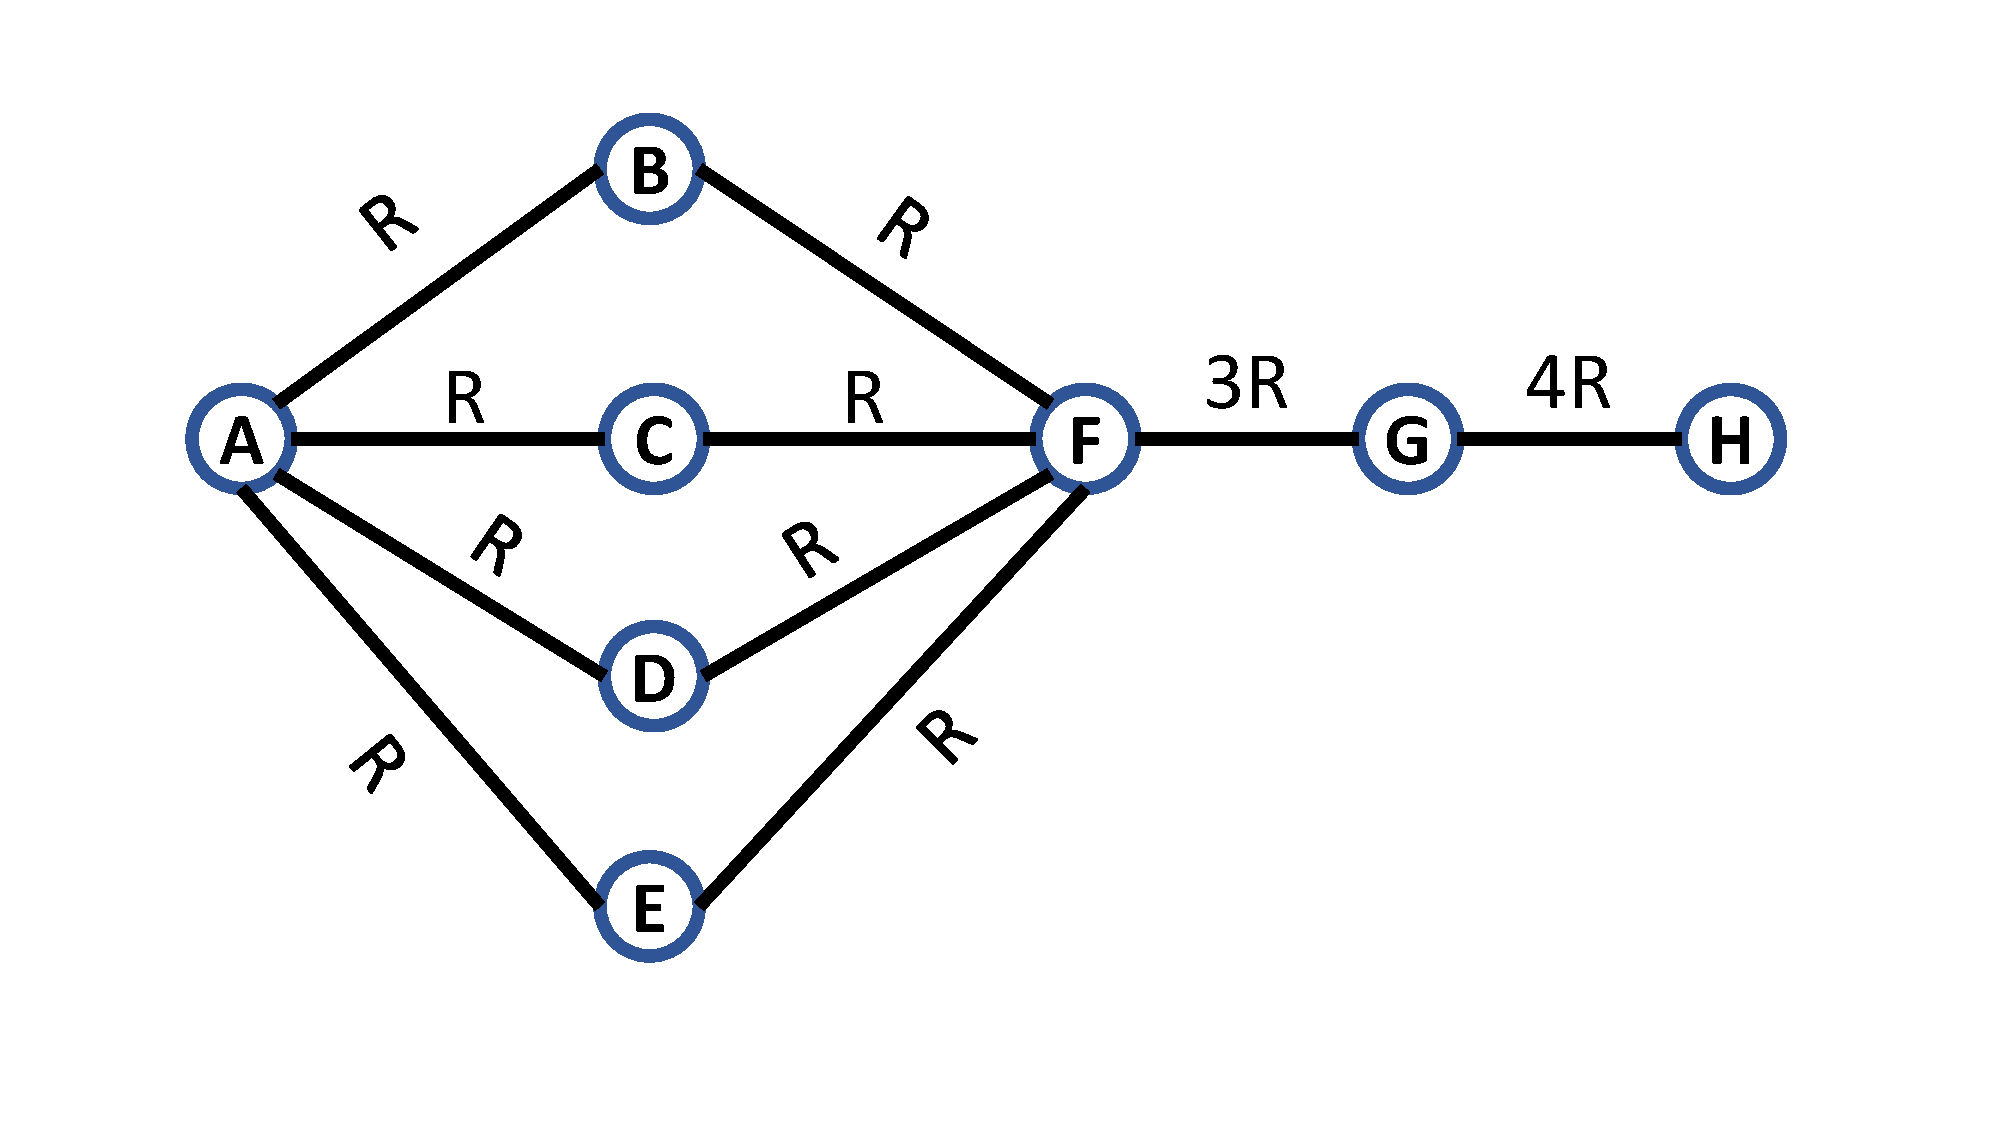
\includegraphics[width=140mm]{Q5}
%\end{figure}
%
%Q5)
%
%In the following network sketch, node A can send packets arbitrarily over each of the three paths to routers R1, R2 and R3 and node B can receive packets arbitrarily too. If each link fails to transmit data with a probability of $p$ independent of the other ones.
%\begin{figure}[ht]
%\centering
%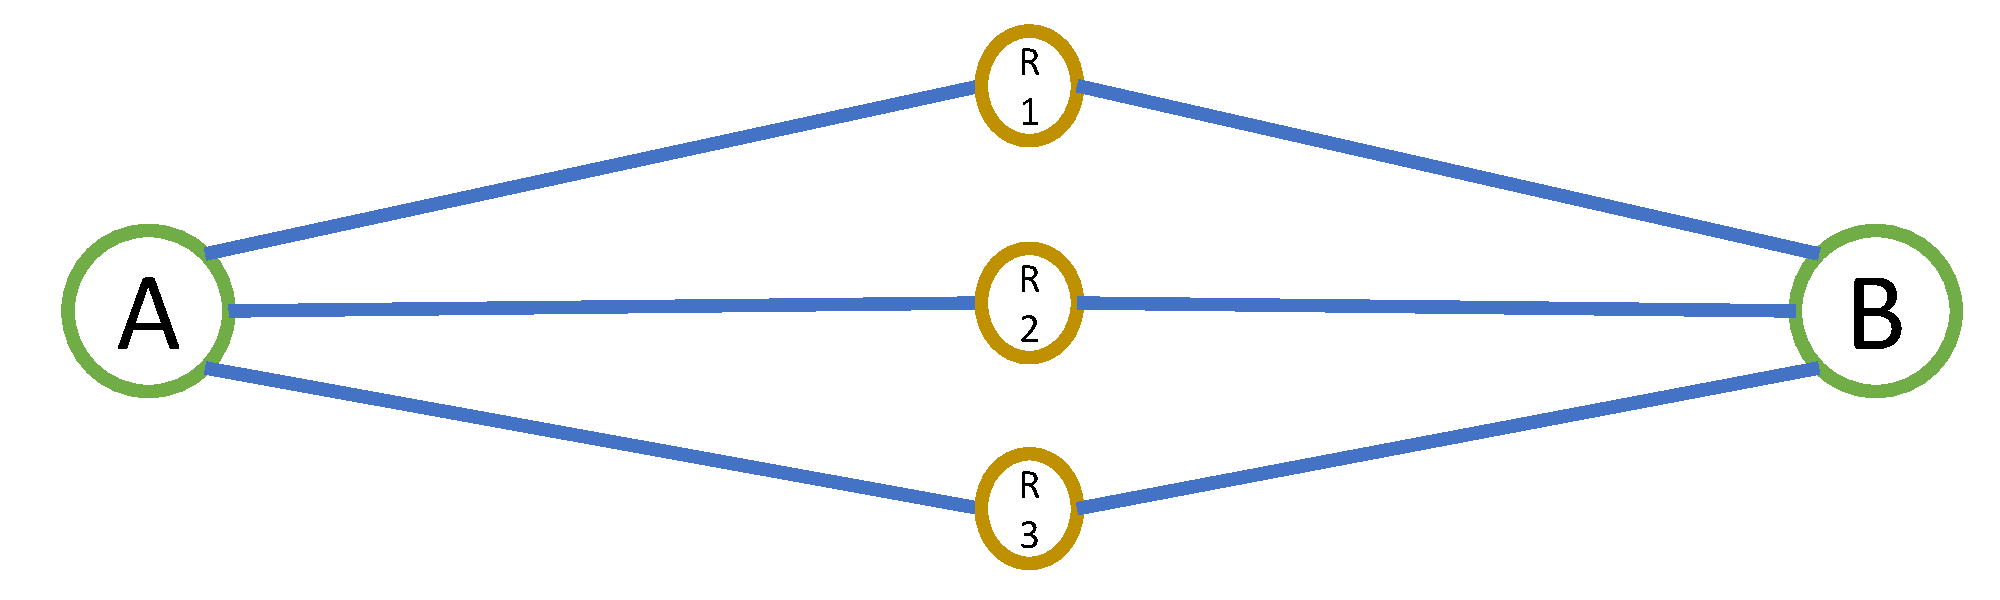
\includegraphics[width=140mm]{p2p_multi}
%\end{figure}
%\begin{enumerate}[label=\alph*-]
%\item
%What is the probability that a packet initiated at node A, finally reaches its destination at node B?
%\item
%If each link has a throughput of $R$, what would be the effective throughput between nodes A and B? (i.e. the throughput that node A actually exploits and senses in transmission to node B; you need to do some probability calculations to obtain the answer!)
%\end{enumerate}
%%\noindent
%%سوال 1) درستی یا نادرستی گزاره های زیر را با بیان دلایل کافی تحقیق کنید.
%%
%%1. برای شدت ترافیک نزدیک به $1$، تاخیر صف
%%\footnote{
%%\lr{Queuing delay}
%%}
%% بسته ها به سمت صفر میل می کند.
%%
%%2. داده برای انتقال از یک هاست
%%\footnote{
%%\lr{Host}
%%}
%% به هاست دیگر، فقط از مجموعه ای از لینک ها می گذرد.
%%
%%3. \lr{API} 
%%مجموعه‌ی قوانینی است که برنامه‌ی سمت فرستنده باید پیروی کند تا اینترنت قادر به انتقال داده به برنامه‌ی مقصد باشد.
%%
%%4. \lr{Packet Switching}
%% پیاده سازی پیچیده تر و پر هزینه تری نسبت به \lr{Circuit Switching} ایجاب می کند؛ ولی در مقابل برای کاربردهای بلادرنگ
%%\footnote{
%%\lr{Real-time}
%%}
%% مناسب تر است.
%%
%%5. یک پروتکل، فرمت و ترتیب پیامهای جابجاشده بین دو واحد مخابراتی را مشخص می کند و به اعمال انجام شده در ارسال و یا دریافت پیام نظارتی ندارد.
%%
%%6. در سمت کاربر، \lr{DSLAM} وظیفه ی جداسازی سیگنال های تلفنی و دیتای اینترنتی را در \lr{cable Internet access} بر عهده دارد.
%%
%%7. در معماری \lr{PON} همه ی بسته های ارسال شده از \lr{OLT} به سمت \lr{Splitter}، در \lr{Splitter} تکثیر می شوند.
%%
%%8. به دلایل اقتصادی، از فیبر نوری نمی توان در شبکه های \lr{long-haul} استفاده کرد.
%%
%%9. لایه‌ی پروتکل فقط در نرم افزار پیاده سازی می‌شود.
%%
%%10. تنها یک پروتکل \lr{IP} وجود دارد و تمام اجزای اینترنت که یک لایه‌ی شبکه دارند، باید از این پروتکل تبعیت کنند.
%%
%%\noindent
%%سوال 2) تفاوت ویروس (\lr{Virus}) و کرم (\lr{Worm}) چیست؟
%%
%%\noindent
%% سوال 3) در یک روتر، بسته
%%\footnote{
%%\lr{Packet}
%%}
%% هایی با طول 8 بیت به ورودی آن ارسال می شوند و نرخ دریافت بسته ها در ورودی از توزیع زیر پیروی می کند:
%%\eqn{
%%f_A(a)={(3.35)^a\cdot e^{-3.35}\over a!}
%%}{}
%%نرخ خروجی بیت در روتر نیز دارای توزیع زیر است:
%%\eqn{
%%R\sim \mathcal{U}(35,40)
%%}{}
%%\indent
%%الف) متوسط شدت ترافیک
%%\footnote{
%%\lr{Traffic Intensity}
%%}
%% را در این روتر محاسبه کنید.
%%
%%\indent
%%ب) اگر چهار بسته به صورت پشت سر هم وارد این روتر شوند، متوسط تاخیر ارسال
%%\footnote{
%%\lr{Transmission delay}
%%}
%% بسته‌ی چهارم چه 
%%\indent
%%میزان خواهد بود؟ (تاخیر ارسال بسته‌ی اول را صفر در نظر بگیرید)
%%\noindent
%%سوال 4) در شبکه ی زیر، اگر احتمال خرابی هر لینک مستقل از سایرین برابر $p$ باشد، احتمال صحت کل مسیر را از $A$ تا $B$ به دست آورید.
%%\begin{center}
%%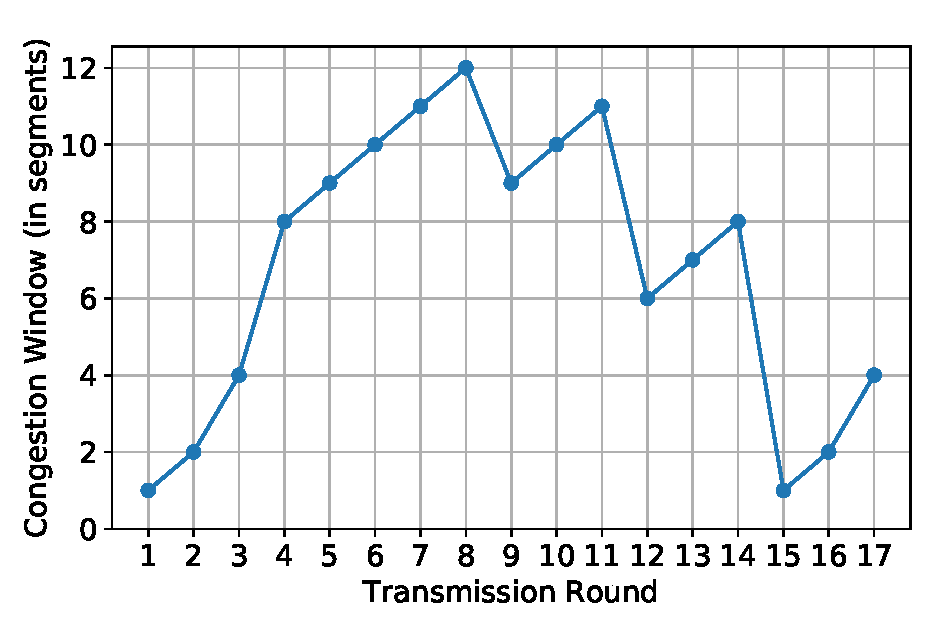
\includegraphics[width=100mm]{Q4}
%%\end{center}
%%سوال 5) در شبکه ای با توپولوژی زیر، در چه صورت و با کدام احتمال حداکثر \lr{throughput} برای مسیر $A-H$ برابر $2R$ می باشد؟ (احتمال خرابی هر لینک مستقل از سایرین برابر $p$ می باشد)
%%\begin{center}
%%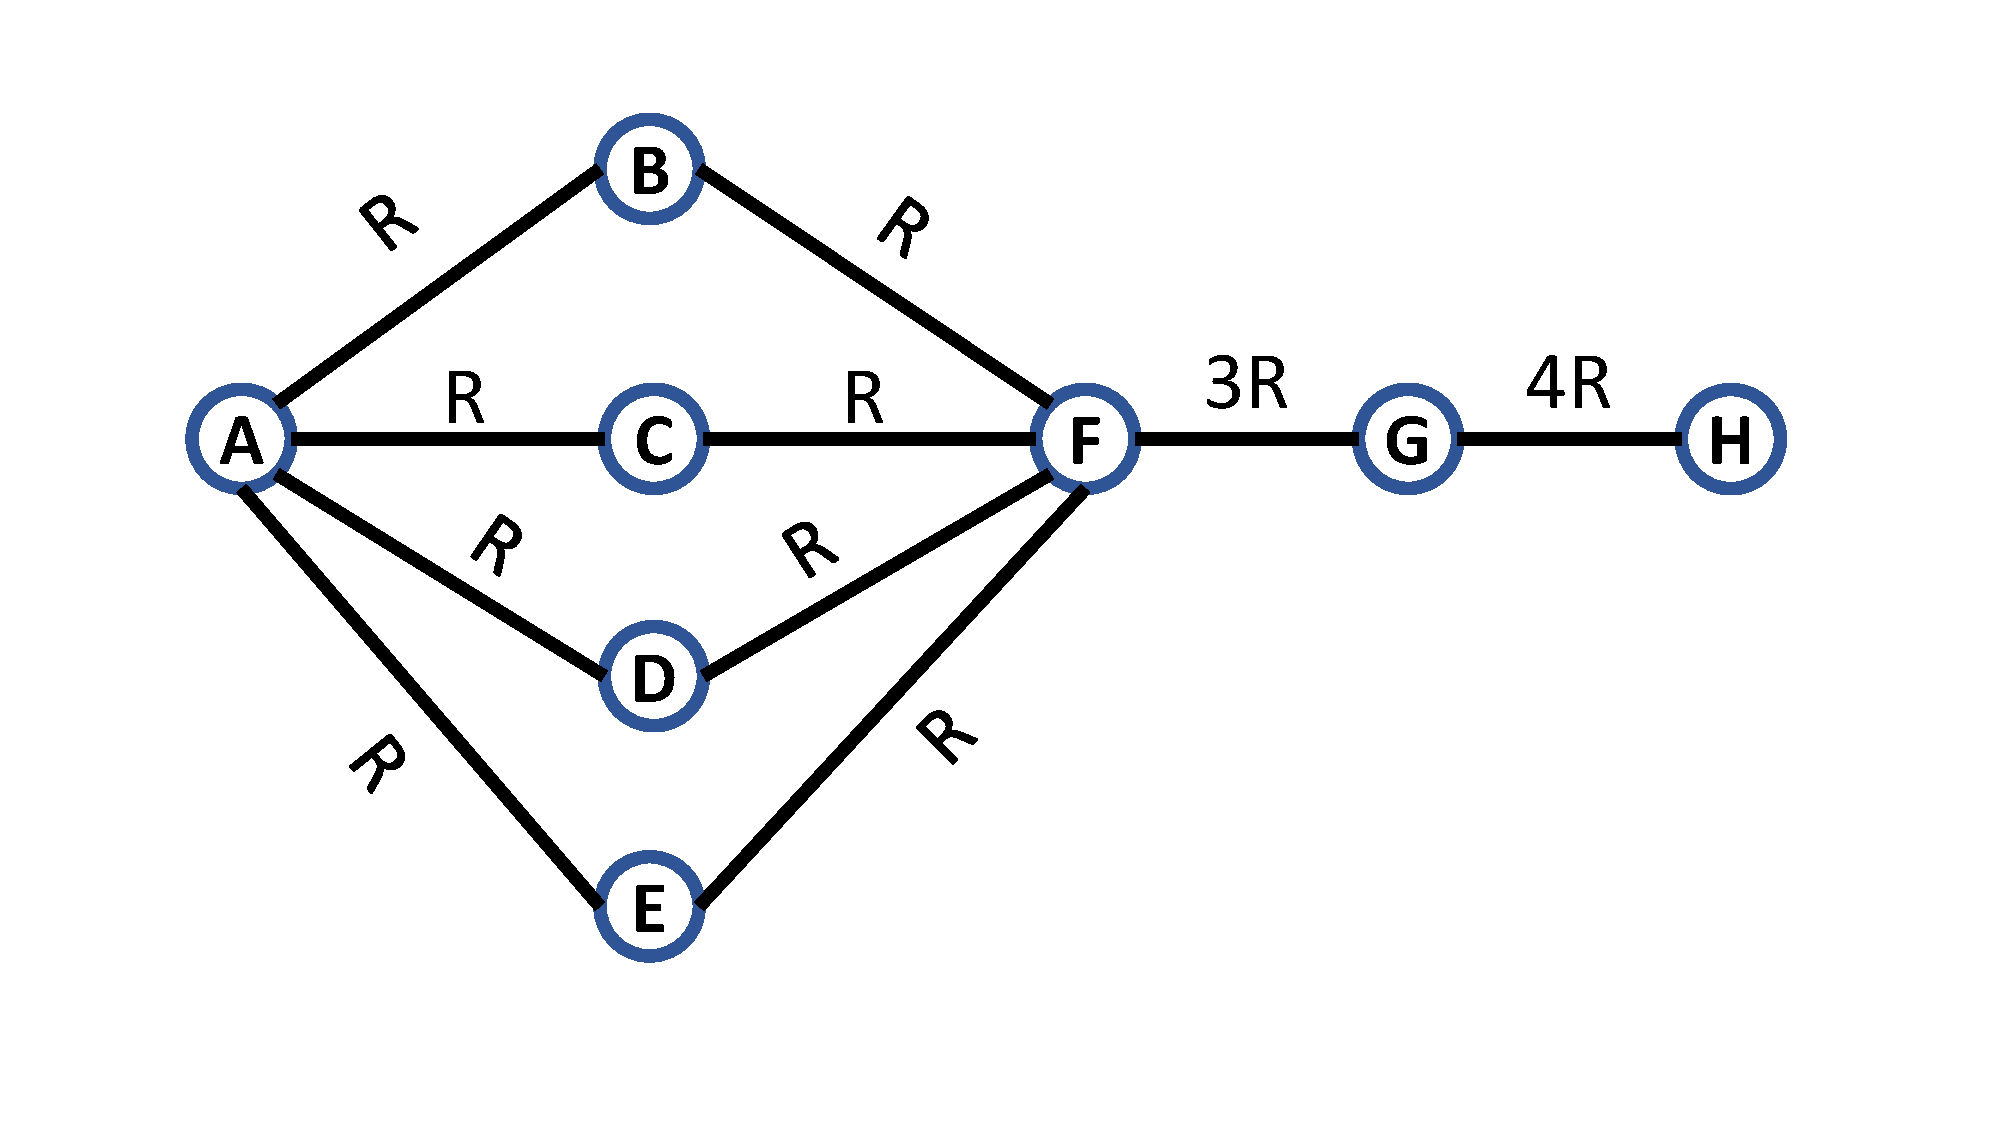
\includegraphics[width=100mm]{Q5}
%%\end{center}
%%\noindent
%%سوال 6) در شبکه‌ی زیر، فرض کنید نرخ ورود بیت به روتر برابر 
%%$1\text{\lr{Mbps}}$
%%، حجم هر بسته برابر 
%%$1\text{\lr{kbytes}}$
%%، تاخیر پردازش هر بسته برابر 
%%$12\text{\lr{msec}}$
%%، طول لینک برابر 200 متر و سرعت انتشار در لینک برابر 
%%$2\times 10^8 \text{\lr{m/s}}$
%% است. همچنین  نرخ خروج بیت از روتر را بینهایت بگیرید.
%%
%%الف) تاخیر ارسال را برای بسته‌ی دهم محاسبه کنید.
%%
%%ب) تاخیر کلی ای را که بسته‌ی دوم در ارسال از \lr{A} به \lr{B} تجربه می کند محاسبه کنید.
%%
%%ج) به مدت چند میلی ثانیه و برای اولین بار، حجم اشغال شده‌ی بافر برابر 
%%$2\text{\lr{kbytes}}$
%% خواهد بود؟ (حالتی که یک بسته بلافاصله وارد بافر می‌شود و تنها بسته‌ی کنونی بافر بلافاصله از آن خارج می‌شود، $1\text{\lr{kbytes}}$ از حجم بافر را اشغال می‌کند. به عبارت دیگر باید مدت زمان غیرصفری محاسبه شود که دو بسته همزمان در بافر حضور داشته باشند)
%%\begin{center}
%%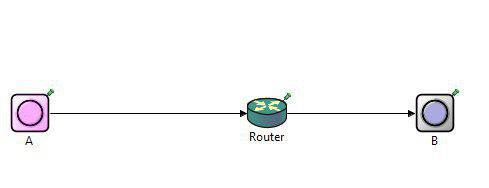
\includegraphics[width=100mm]{Q6.jpg}
%%\end{center}
\end{document}